\TransitionFrame{caratteristiche dei manipolatori continui}

\begin{frame}{Terminologia}
\begin{columns}
\begin{column}{0.5\textwidth}
\begin{itemize}
    \item<1-> \textcolor{yellow}{continuum robot}
    \item<2-> hyperredundant robot
    \item<3-> pseudocontinuum robot
\end{itemize}
\end{column}
\begin{column}{0.5\textwidth}
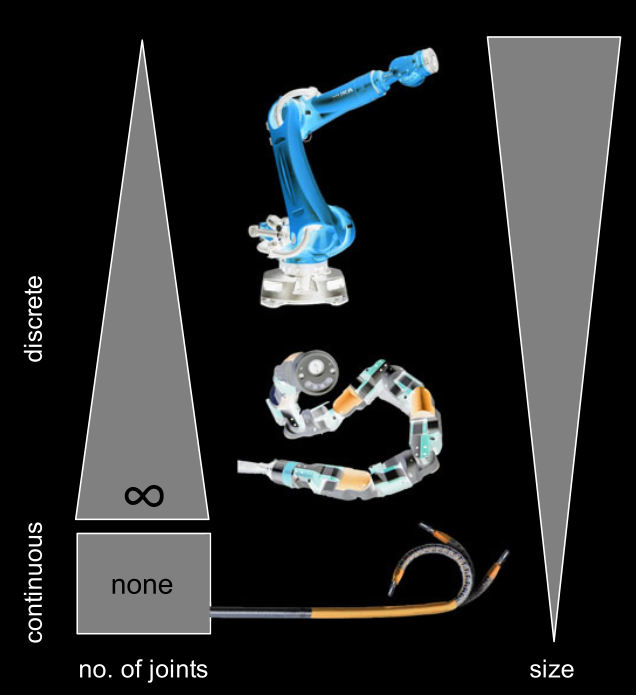
\includegraphics[width=\textwidth]{slide_studio/img_terminologia/terminologia.png}
\end{column}
\end{columns}

\BReference{Continuum Robots for Medical Application: A Survey}{Burgner-Kars, Rucker}{2015}

\note{
Continuum robot $\to$ struttura attuabile il cui materiale costitutivo forma una curva differenziabile. Definizioni alternative: $\infty$-DOF, senza link rigidi, senza giunti identificabili. \\

Hyperredundant robot $\to$ numero elevato di link e giunti. Il materiale costitutivo forma una linea spezzata che approssima una curva differenziabile con precisione arbitraria. \\

Pseudo-continuum robot $\to$ sia link rigidi che elementi in grado di piegarsi in modo continuo.
}
\end{frame}

